\section{Application Characterization}
\label{sec:characterize-app}

  We now turn to measurements of specific popular iOS and Android applications. 
  When users install apps, they grant them Internet access without detailed knowledge of how that access will be used, including {\it how much} data is sent or accessed, {\it what} data is sent,  or {\it with whom} the app communications.
  ``How much'' is important to conserve both bandwidth caps and battery capacity: an app which consumes or produces too much data will waste bandwidth resources, while an app which consumes or produces data too frequently will prevent the device radio from going idle to save power.
  ``With whom'' is important to protect users from excessive tracking -- the more organization's servers an app connects to, the more organizations which are able to track user behavior, location, or other private data.
  Finally, ``what data'' is important because apps may unnecessarily leak personally identifiable information (PII) such as user email address, IMEI, contact information, or other stored data either to the app provider or worse, to any eavesdropper on a public WiFi connection.
  We  report on our findings in all three of these dimensions for the iPhone and Android apps in our study.

\subsection{Bandwidth and Radio Usage}

  {\bf In the Wild.}
    \begin{itemize}
      \item Stats on how much bandwidth each user used; time of day; how frequent...
    \end{itemize}

  {\bf Android Apps.}
    To dig in to the root cause of these usage patterns, we also did an `app-by-app` analysis of network usage to see if most bandwidth consumption/radio time was the result of a few heavy applications, with most applications relatively idle, or whether usage was divided amongst all applications equally.
    In Figure~\ref{fig:app-by-app-usage}, we plot the CDF of total bytes transferred by each app in our study, one line for the top-100 Google Play apps we tested manually, and another for the top 2000 apps, tested automatically, from a third-party market.
    We see that...\tbd{Amy...}
    We see that in general, more bytes are received than sent (289711536 vs 3040151). This is probably due to advertising, where the size of the requests is much smaller than the advertisements received. Indeed, most of the applications contacted Google, through AdMob. A few third-party advertising servers were also contacted. 
    
Applications in general fit their expected bandwidth usage(Spotify, predictably sent the most bytes (sent 318980 received 12108538) and a notepad application used the least (sent 414 received 262). However, some games used a surprisingly large amount of bandwidth (The Simpsons(TM): Tapped Out 149291 88932890 and Jurassic Park(TM) Builder
 312912 127163147 (These two received the most bytes)). Ludia games in particular used an unusually large amount of bandwidth. Ludia's Jurassic Park(TM) Builder ran for 13 minutes, and Ludia's Family Feud and Friends Free ran for 7 minutes. Ludia's Jurassic Park(TM) Builder was 38.1 MB  and Ludia's Family Feud and Friends Free was 27.6 MB. This may be because of game updates (for example, a lot of these games may have released more in-game content for Easter, new textures, new models, etc.) These applications were tested before Google updated its Play Developer Program Policies on May 1, 2013 to say, "an app downloaded from Google Play may not modify, replace or update its own APK binary code using any method other than Google Play's update mechanism." However, companies may still subvert this new policy by pushing textures and other in-app purchases aren't necessarily modifying the apk binary code, but still use excessive bandwidth. 
 
In terms of categories, games had the most variable amount of usage. Music/video applications were consistently the biggest users of bandwidth. Productivity/tool apps tended to use the least.

    Regarding radio usage,...\tbd{Do we even have time to do this? I don't remember the exact metrics we used for the MobiSys submission.}

  {\bf iPhone Apps.}

\subsection{Third Party Servers}
  Many free applications support themselves financially by serving ads or providing resources for third parties to track user behavior.
  We now explore how many servers are contacted by a given app (\ie{} how many providers are tracking a user with this app) -- most of these typically for ads, tracking, or analytics -- as well as how much data is transferred to and from these servers (\ie{} how much does this traffic impact the user's data cap?).

  {\bf In the Wild.}
  We first consider the overall impact of these ads, analytic, and tracking services on typical user behavior in our IRB study...
  \tbd{Ashwin...}

\begin{figure}[t]
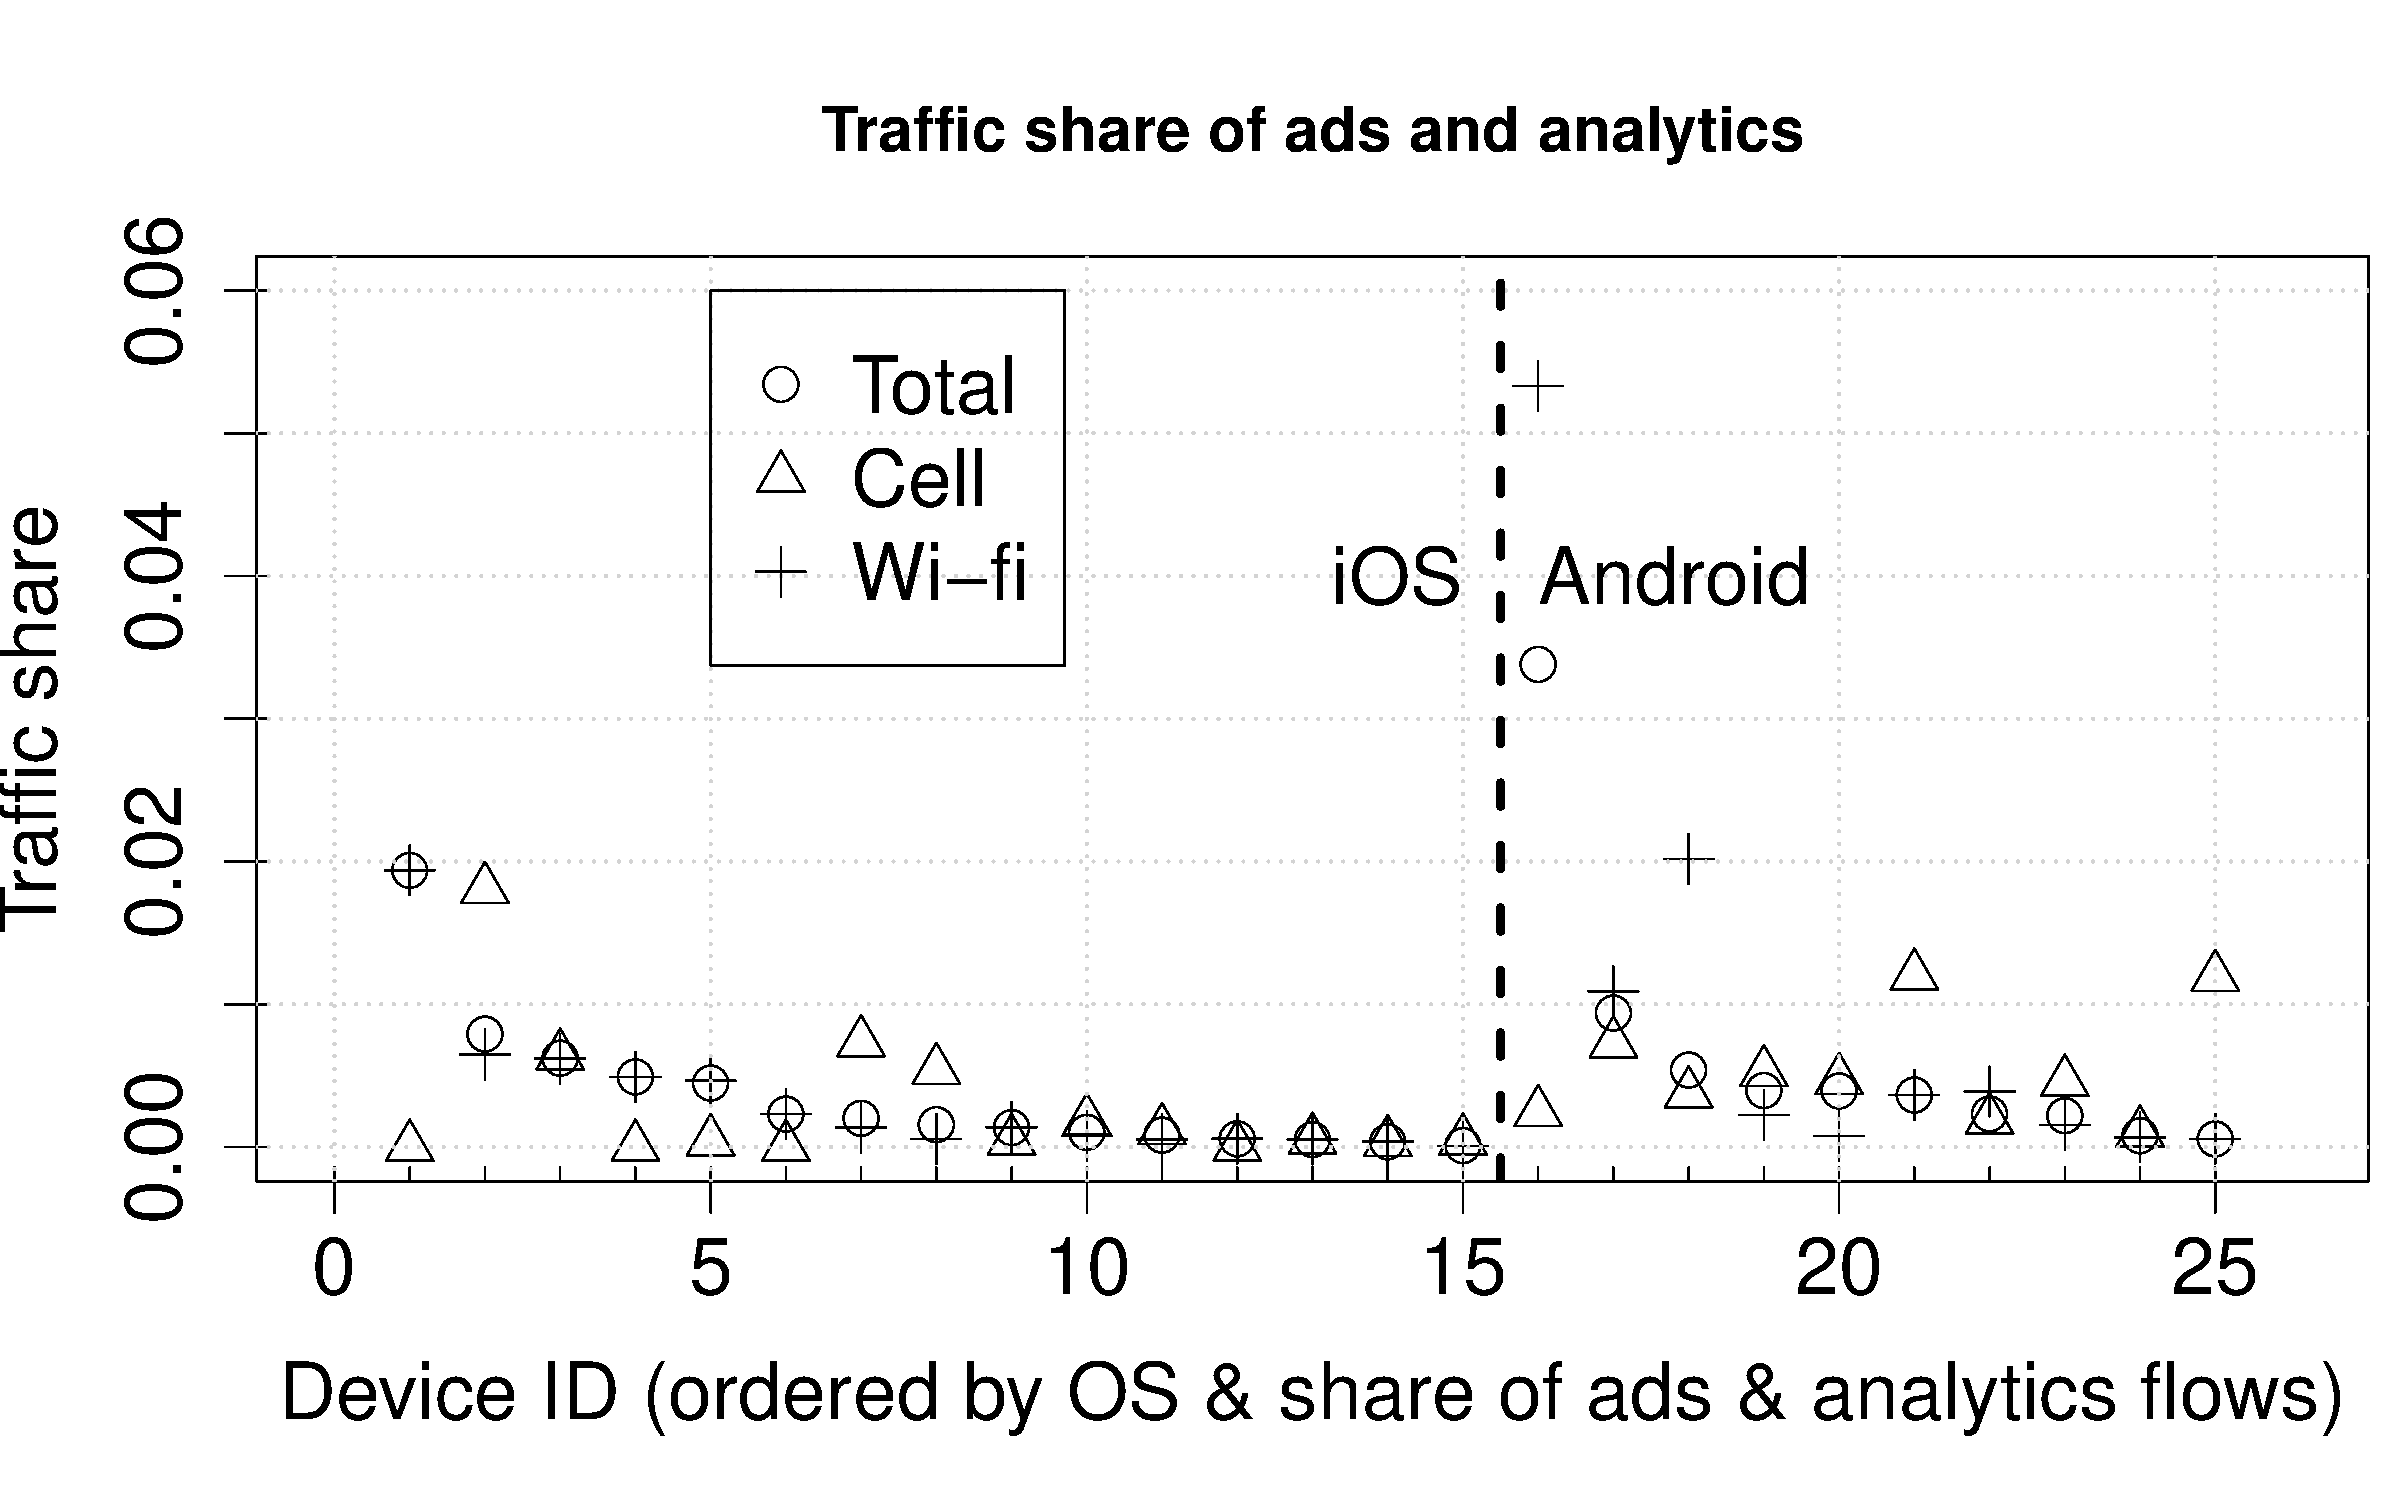
\includegraphics[width=\columnwidth]{plots/ad_share_bytes.pdf}
\caption{Fraction of traffic volume because of Ads and Analytics. \emph{\tbd{Check for id1 and id25}}}
\label{fig:description}
\end{figure}

\begin{figure}[t]
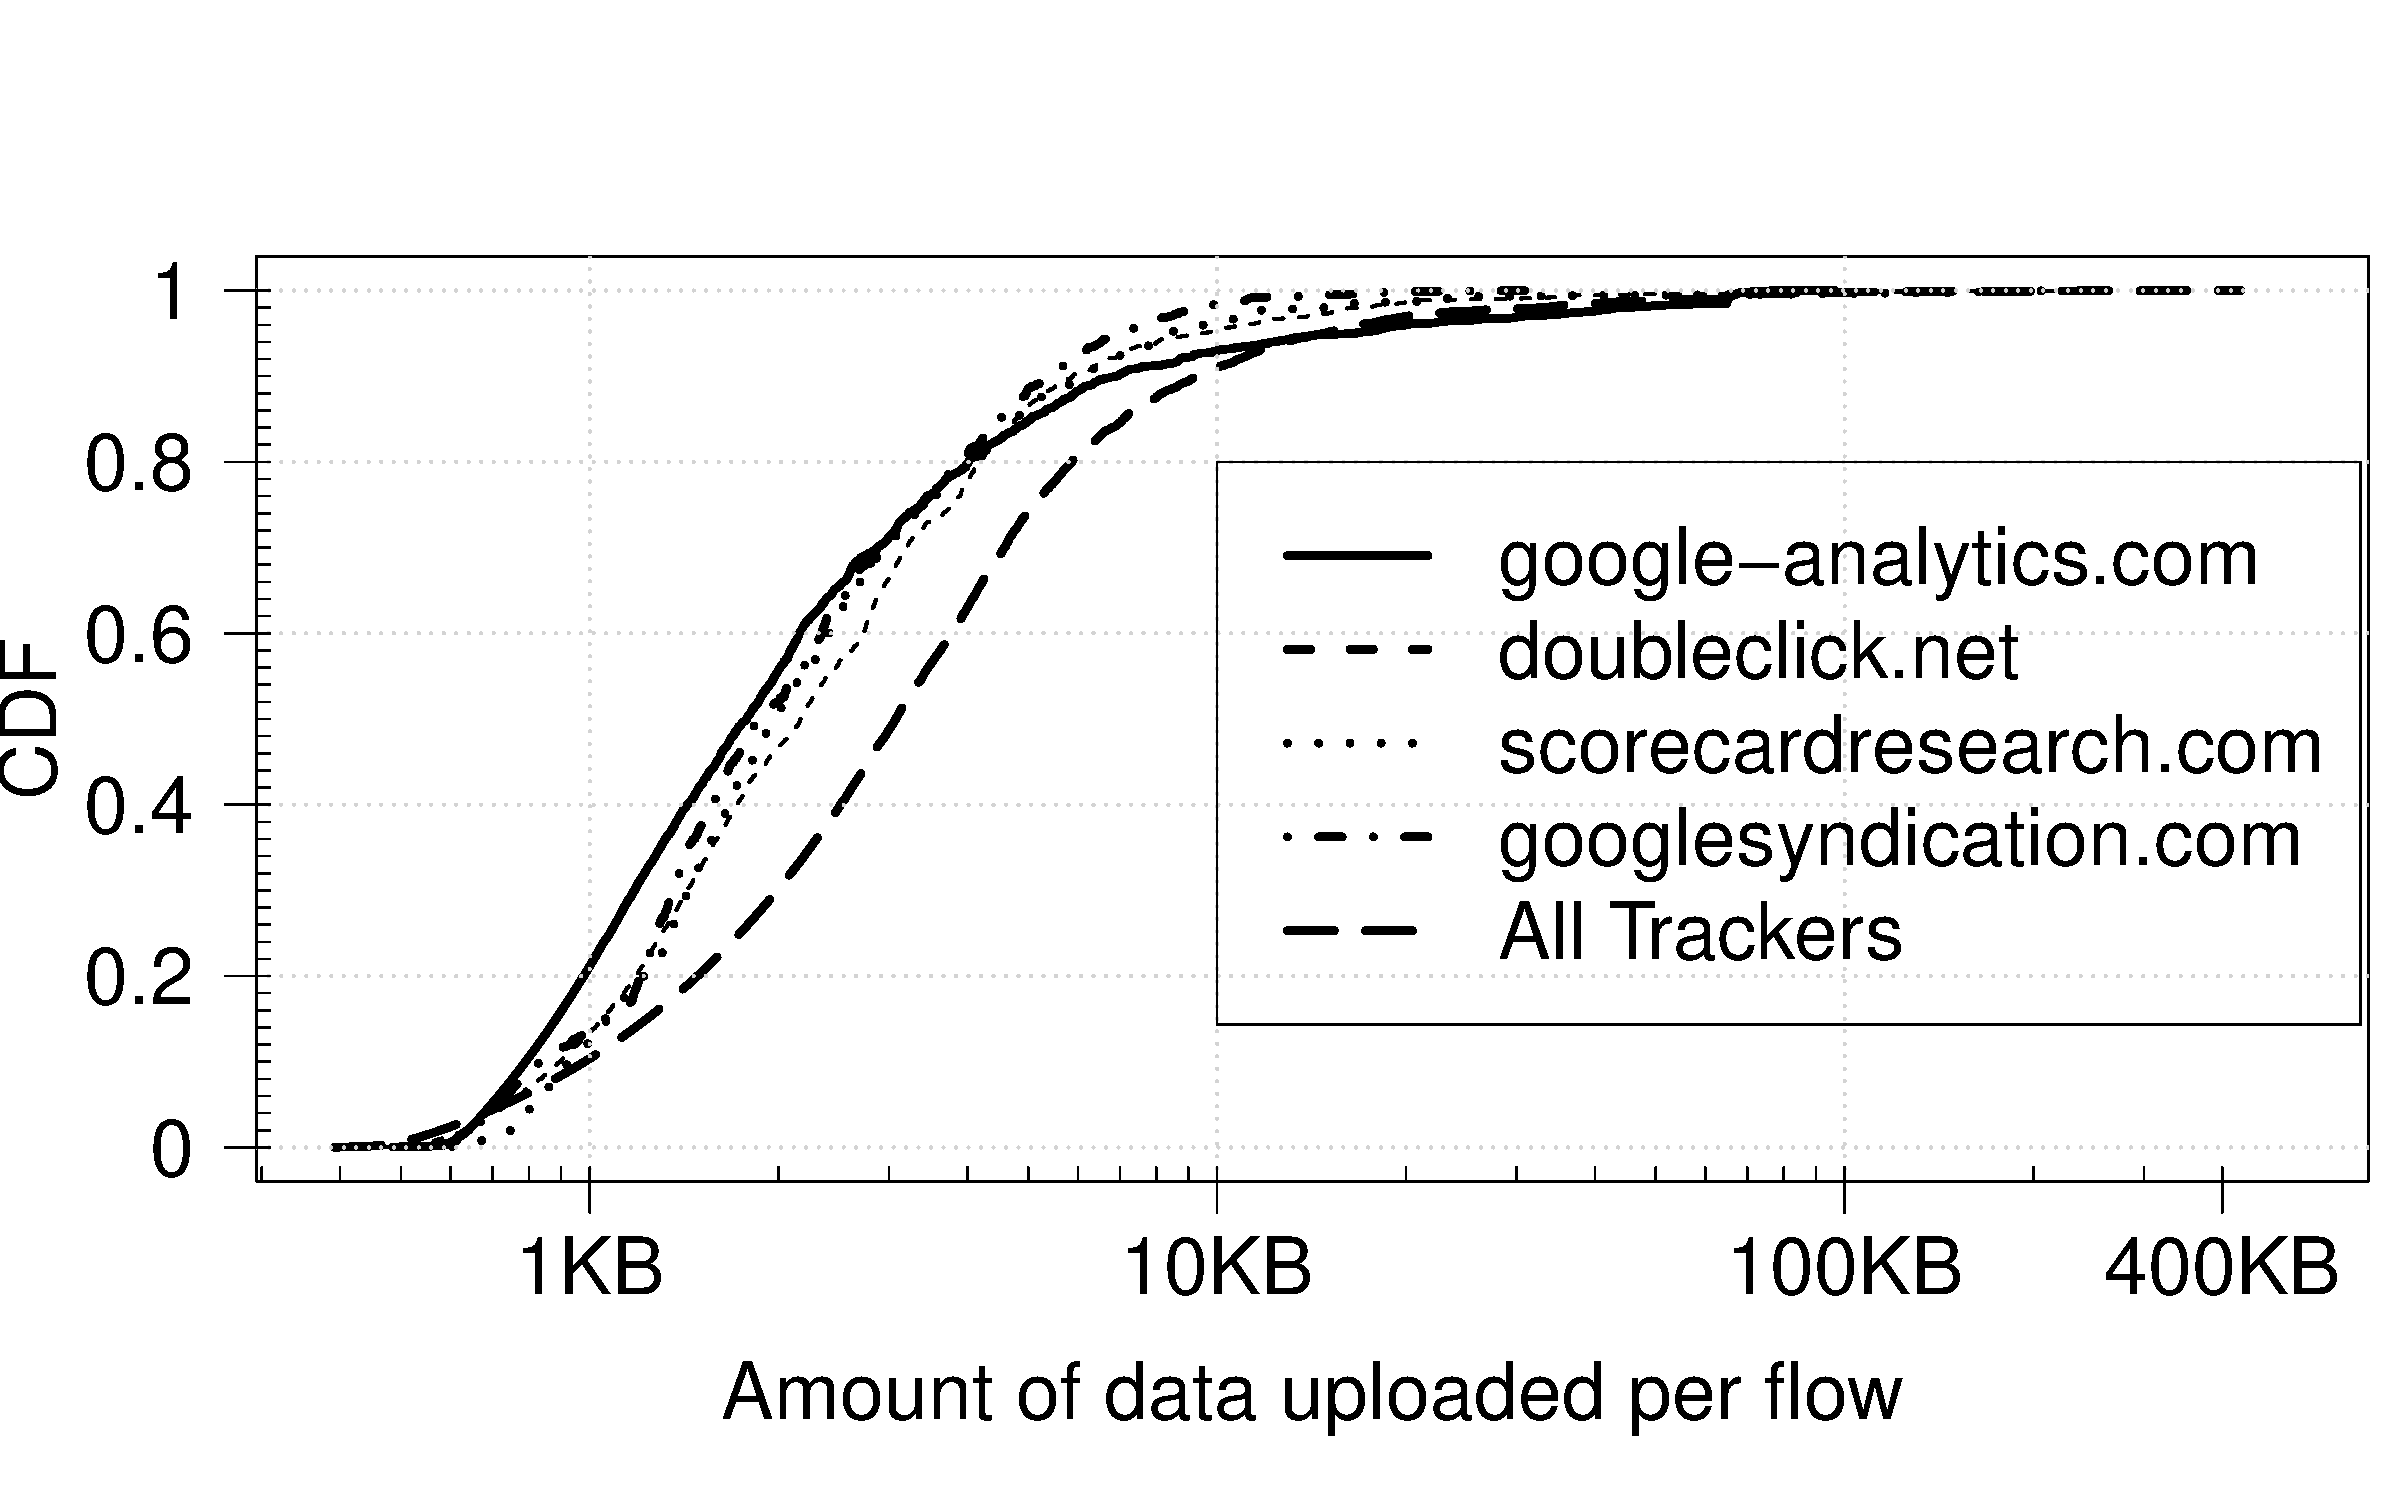
\includegraphics[width=\columnwidth]{plots/distrib_ad_uploads.pdf}
\caption{Distribution of bytes uploaded by ads and analytics sites. \emph{The distribution of bytes uploaded by all ads and analytics sites and the top four ads sites based on traffic volume across all users}.}
\label{fig:description}
\end{figure}

\begin{figure}[t]
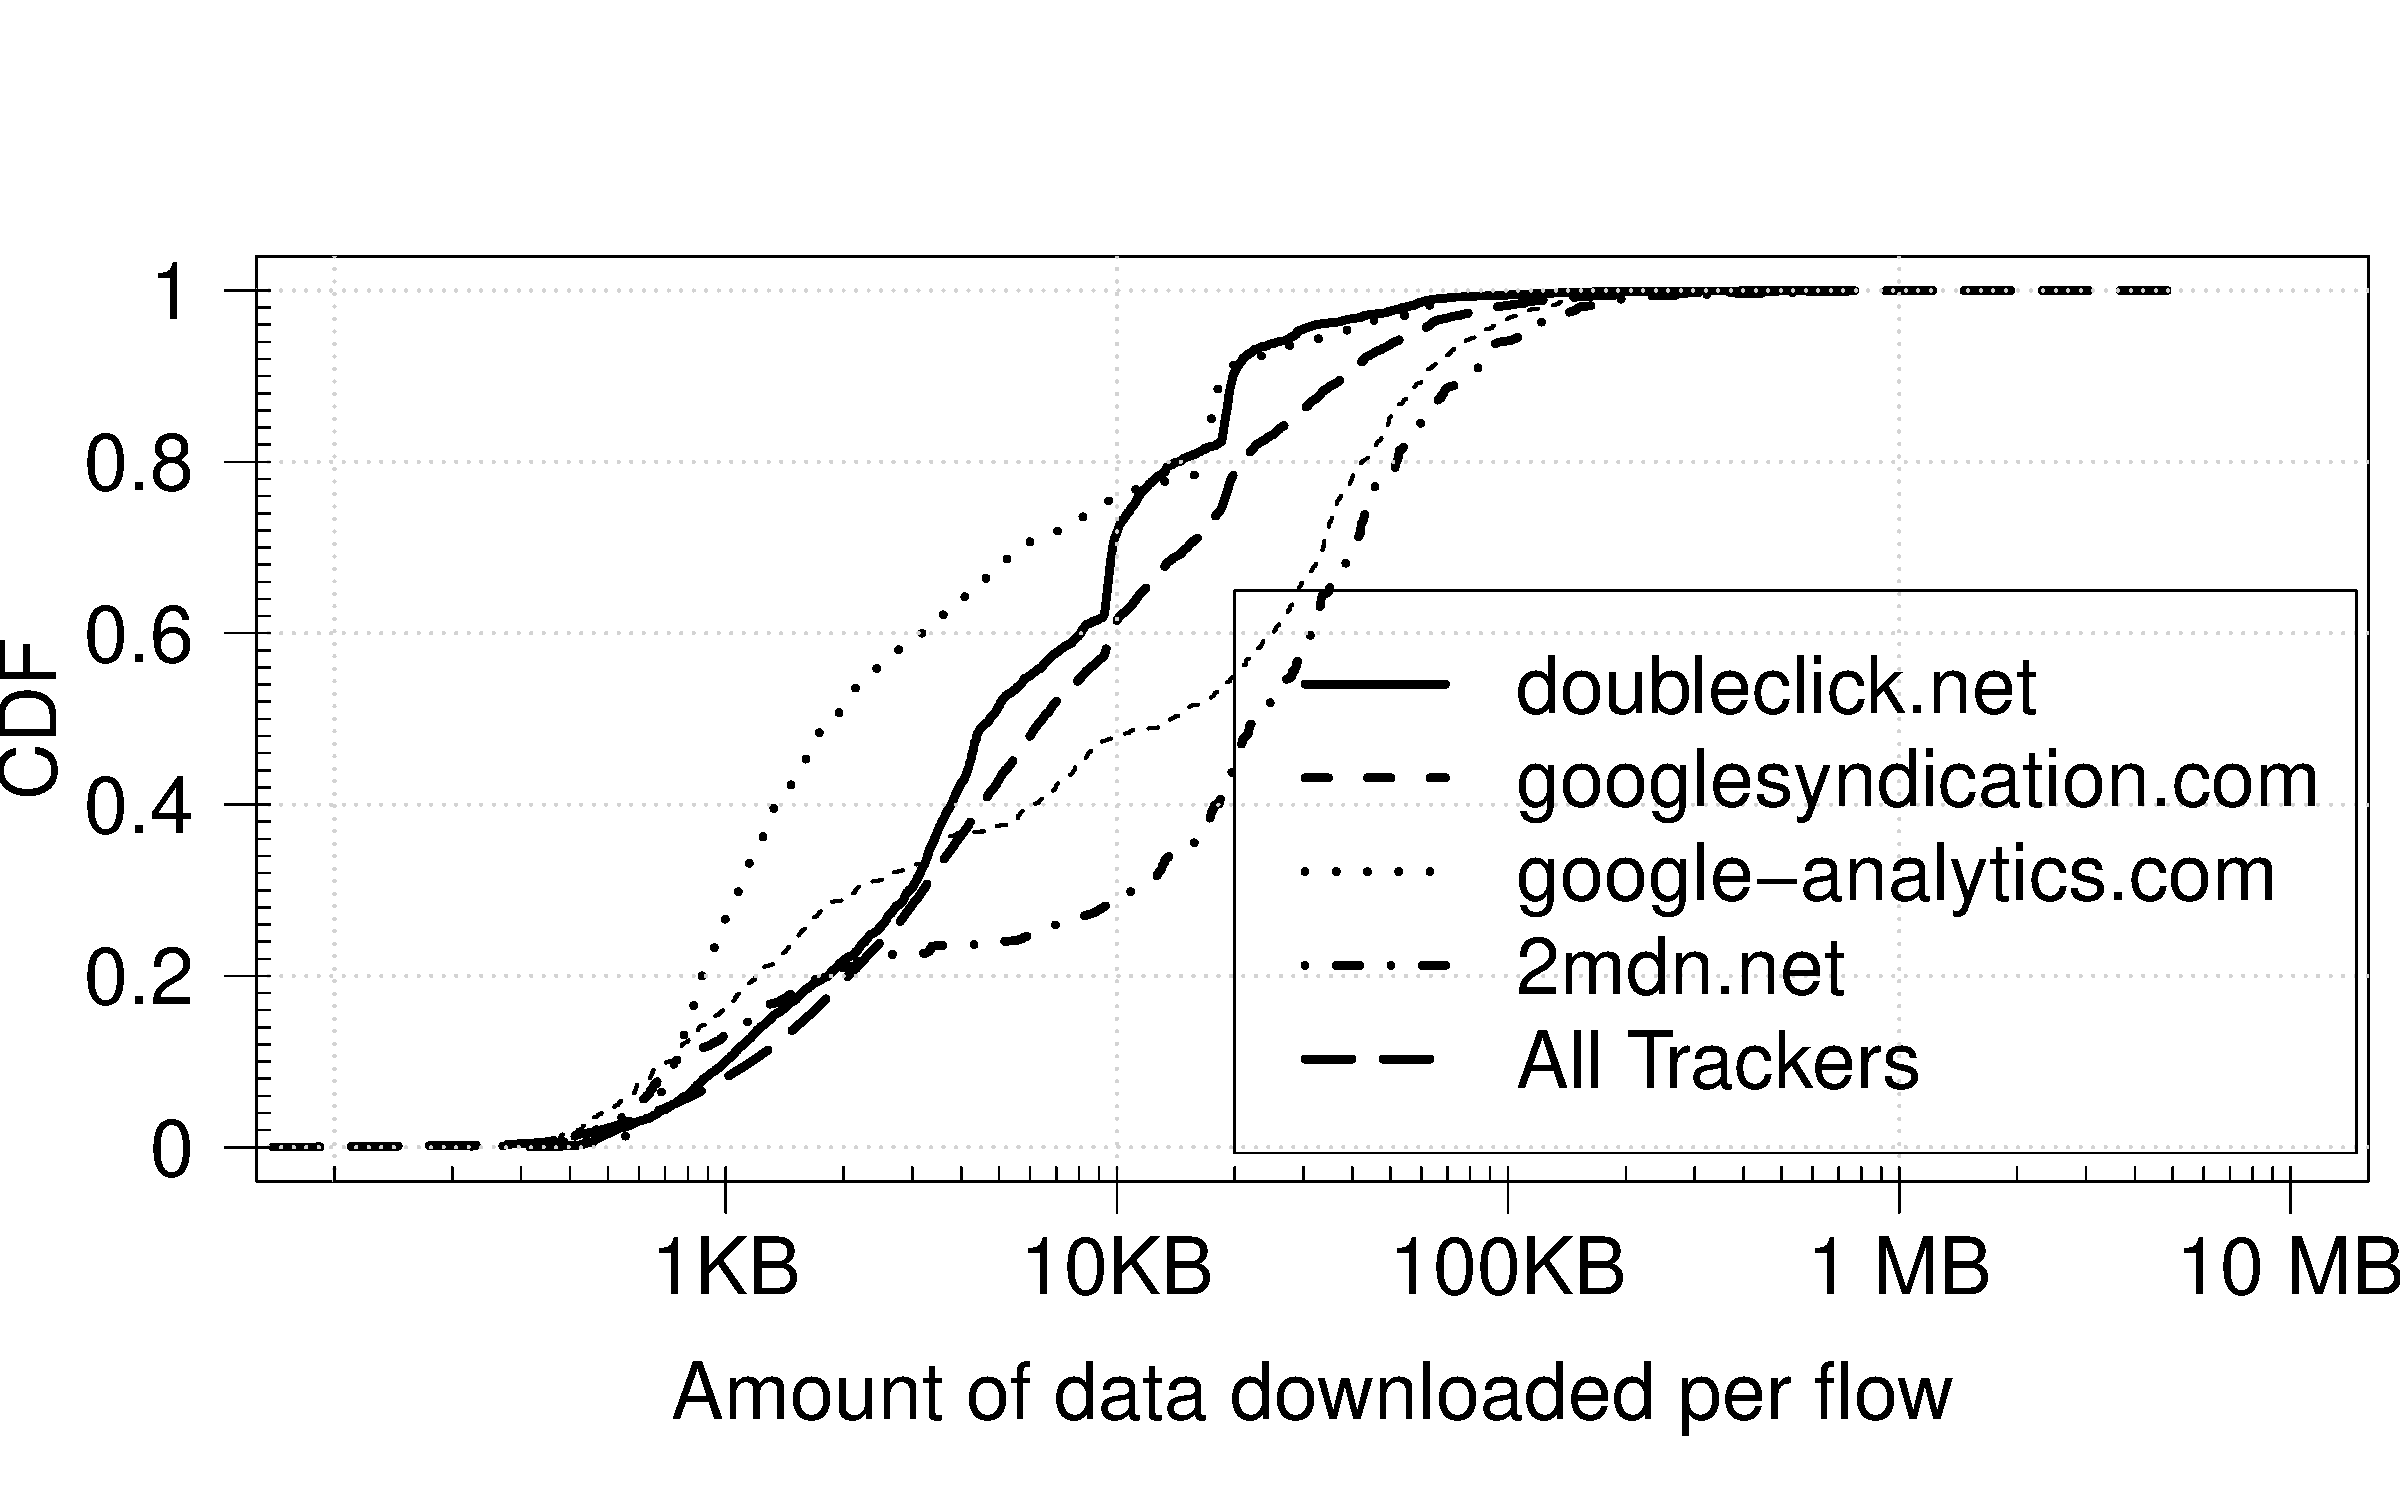
\includegraphics[width=\columnwidth]{plots/distrib_ad_downloads.pdf}
\caption{Distribution of bytes downloaded by ads and analytics sites. \emph{The distribution of bytes uploaded by all ads and analytics sites and the top four ads sites based on traffic volume across all users}.}
\label{fig:description}
\end{figure}

\begin{table}[t]
\centering
\begin{small}
\begin{tabular}{|p{0.35\columnwidth}|p{0.1\columnwidth}|p{0.15\columnwidth}|p{0.1\columnwidth}|}
\hline
\multirow{2}{*}{\bf Tracker} & \multicolumn{3}{c|}{\bf Number of devices tracked}\tabularnewline
\cline{2-4}
   &  {\bf Total} & {\bf Android} & {\bf iOS} \tabularnewline
\hline
doubleclick.net & 25 & 11 & 14 \tabularnewline
\hline
google-analytics.com   & 25 & 11 & 14 \tabularnewline
\hline
googlesyndication.com  & 22 & 10 & 12 \tabularnewline
\hline
admob.com  & 21 & 10 & 11 \tabularnewline
\hline
scorecardresearch.com &  21 & 10 & 11 \tabularnewline
\hline
2mdn.net  &  20 & 9 &  11 \tabularnewline
\hline
atdmt.com  & 18 & 9 &  9 \tabularnewline
\hline
imrworldwide.com & 18 &  9 &  9 \tabularnewline
\hline
flurry.com & 17 & 7 &  10 \tabularnewline
\hline
googleadservices.com  & 17 & 8 &  9 \tabularnewline
\hline
\end{tabular}
\end{small}
\caption{The top 10 ads and analytics sites that tracked the devices in our dataset.
\emph{Two trackers, \emph{doubleclick.net} and\emph{google-analytics.com}, were tracking all the 25 devices in our dataset.}}
\label{tab:top_trackers}
\end{table}


\begin{table*}[t]
    \centering
    \begin{tabular}{l|l|l|l|l|l|l|l|l|l}
       Dataset&Platform&\# Apps&Email&Location&Name&Password&Android ID&Contacts&IMEI\\
       \hline
       \hline
       Google Play&Android&100&3 (3\%)&10 (10\%)&2 (2\%)&1 (1\%)&21 (21\%)&0 (0\%)&13 (13\%)\\
       \hline
       Third Party&Android&908&1 (0.1\%)&32 (3.5\%)&2 (0.2\%)&0 (0\%)&95 (10.4\%)&4 (0.4\%)&48 (5.3\%)\\
       \hline
       App Store&iPhone&100&?&?&?&?&?&?&?\\
    \end{tabular}
    \caption{\label{tbl:pii}Summary of personally identifiable information leaked in plaintext (HTTP) by Android and iPhone apps.}
  \end{table*}
  

  {\bf Android Apps.}
  When we inspect the data from our controlled study, we see that some apps contact a large number of external servers while others contact significantly fewer.
  In Figure~\ref{fig:android-cdns}, we show both the total number of servers contacted (solid lines) as well as the number of organizations contacted (dotted lines) for both the top-100 Google Play dataset and the top-2000 third-party dataset.
  To quantify ``organizations contacted'', we performed whois lookups on all servers contacted and mapped them to an organization name, allowing us to tighten our upper bound on the number of companies/entities able to track the user through a single app.
  Returning to the figure, we see...~\ref{fig:android-cdns}...\tbd{Amy...}
After doing whois lookups on all contacted servers, we categorized by hand each server.
For all of the hundred apps, we broke down the 51 servers that each visited into these categories:
\begin{itemize}
   \item 3 Advertising
   \item 1 Analytics
   \item 6 CDN
  \item 10 Hosting
  \item  1 IANA
  \item  1 ISP
   \item 3 Network
  \item 23 PrivateCompany
   \item 3 RegionalInternetRegistry
\end{itemize}
   For all of the third party apps, we broke down the 96 servers that each visited into these categories:
\begin{itemize}
\item      4 Advertising
 \item   1 Analytics
 \item   8 CDN
 \item  31 Hosting
 \item   1 IANA
 \item   2 ISP
\item    8 Network
\item   37 PrivateCompany
 \item   4 RegionalInternetRegistry
 \end{itemize}
   
   Words with Friends contacted an astounding 21 servers:
\begin{itemize}
\item    1 Advertising
\item    3 CDN
\item    7 Hosting
\item    1 IANA
\item    1 Network
\item    5 PrivateCompany
\item    1 RegionalInternetRegistry
\end{itemize}
ooVoo Video Call also contacted 21 servers, and interestingly, contacted Fastly, an analytics company. 
\begin{itemize}
\item    2 Advertising
\item    1 Analytics
\item    5 CDN
\item    1 Hosting
  \item  1 IANA
\item    1 ISP
 \item   1 Network
\item    8 PrivateCompany
  \item  1 RegionalInternetRegistry
\end{itemize}

Small practical apps such as PhotoGrid - Collage Maker and ColorNote Notepad Notes generally did not contact many servers at all.
\begin{itemize} 
\item com.socialnmobile.dictapps.notepad.color.note
\item 10.11.4.21	Internet Assigned Numbers Authority
\item 128.208.4.1	University of Washington
\item 74.217.75.7	Internap "
\item com.roidapp.photogrid
\item 10.11.4.22	Internet Assigned Numbers Authority
\item 128.208.4.1	University of Washington
\item 173.194.33.45	Google Inc."
\end{itemize}

  {\bf iPhone Apps.}
  \tbd{Shen...}

\subsection{Personally Identifiable Information}
 
  Finally, we turn to information leaked by individual applications. We do not report on data leaked for our real users here, but only the data leaked by our controlled apps in isolation.
  We created fake user accounts on the test phones for a fake user named ``Tess Droid'', with fake contact information and fake Twitter and Facebook accounts. 
  We were then able to check that none of this data ever was released over the network, either in plaintext (HTTP) or encrypted (HTTPS, see \S\ref{sec:bumping}).
  
  We consider data to be `leaked' when any personally identifiable information -- email address, phone number, IMEI number -- is sent across the network under HTTP or HTTPS.
  Some of this information may be relevant to the app -- \eg{}, many apps legitimately require email access. 
  However, none of this information should ever travel across the network in plaintext (HTTP), which we see violated in serveral cases.

  In Table~\ref{tbl:pii}, we see the type of PII leaked for both Android and iPhone apps.
  For Android apps, IMEI and Android ID are the most commonly leaked forms of PII in both the Google Play and third-party dataset.
  Although not popularly thought of as ``private'' data, each of these identifiers are globally unique: IMEI is a unique identifier tied to a phone, and an Android ID is an identifier tied to a user's Google Account, used across many services on the Internet. 
  Consequently, either of these datapoints can be used to track or correlate a user's behavior across all sites the user visits that sell or collaborate with tracking data: a user's behavior on one site can easily be linked to their behavior on any other site they visit.
  With Android ID being tracked by between 10 and 20\% of apps in our study, and IMEI being tracked by between 5\% and 13\% of apps in our study, this suggests that global user tracking across collaborating services can be easily achieved today just by using this identifier.
  \tbd{...}

  Other informaiton like contacts, email, and passwords were rarely leaked in the clear, but all were leaked on occaision, suggesting that stricter monitoring of Android app behavior is needed -- contrastingly, no iPhone apps (which are manually given clearance by Apple before hitting the iPhone store) leaked passwords in plaintext~\tbd{is this true.}

  Moving to iPhone apps, \tbd{...}
%\subsection{Characterize Facebook Applications}

%Why Facebook was chosen?

%What do we observe ?

%What do we see in the User Agent Fields. 


